\chapter{MDAC Design and Integration}
After successfully simulating the design with ideal circuit blocks, the next step was to perform the transistor level design of the MDAC. The MDAC is one of the most important blocks in a pipelined ADC design. The accuracy of the closed-loop gain directly affects the accuracy of the downstream ADC. In addition, the overall power consumption and noise power is generally dominated by the contributions from the MDAC, so careful design of the MDAC is required in order to obtain high accuracy and low power consumption. From Section \ref{sec:mdacoperation}, the MDAC consists of an OTA along with a capacitive feedback network. Since the feedback network and OTA parameters had already been specified in Section \ref{sec:designparameters}, the main design task was to meet the required specifications using a transistor level design. This chapter will begin with a discussion of the chosen OTA architecture, as well as the main design knobs used to obtain the required OTA specifications. Next will be a high level overview of the biasing and CMFB networks used to obtain the OTA operating point. Following this is a discussion of the simulation methods used and some design challenges that had to be overcome after initial simulations. This chapter then moves on to a presentation of the simulation results of the OTA. Finally, the performance results of the full ADC with the OTA integrated are presented and a final FOM of the design is calculated.
\section{OTA Design}
From Section, \ref{sec:idealotaparams}, in order to achieve the required static and dynamic errors, a loop gain of \SI{48}{\decibel} and a loop crossover frequency of \SI{22.1}{\mega\hertz} was required. The main factor driving the choice of OTA topology was the large gain required. The maximum gain in almost all OTA architectures is set by the intrinsic gain, \gmgds\spc or \gmro, of its transistors. In order to achieve an open-loop gain of \SI{73}{\decibel} using a topology with a gain of approximately $(g_mr_o)^2$, an intrinsic gain of approximately \SI{36}{\decibel} would be required. Assuming minimum channel length devices, intrinsic gains this large would not be achievable. If, however, a topology with a gain of approximately $(g_mr_o)^3$ was used, the required intrinsic gain drops to approximately 16. An intrinsic gain of 16 is attainable using minimum channel length devices, so the investigation was limited to topologies with a gain proportional to $(g_mr_o)^3$. Two topologies that fit this requirement are a triple cascoded topology and a two-stage topology with a cascoded first stage. In general, two stage designs require pole splitting to maintain stability, which causes the dominant pole to shift lower. These concerns are not present with cascoded designs, since the nondominant pole is generally close to the transit frequency. This means that higher bandwidths are easier to obtain using a single triple cascoded stage. In addition, using a single stage generally consumes less power, since each stage requires its own bias current. The main reason why many designs do not use a triple cascoded topology is their extremely limited output swing. For a triple cascoded differential topology, the output voltage range is approximately:
\begin{equation}
\label{eq:triplecascodeoutputswing}
-(V_{dd} - 7V_{ov}) < V_{out} < (V_{dd} - 7V_{ov})
\end{equation}
where $V_{ov}$ is the overdrive voltage of the transistors. For many low-voltage processes, this limitation prohibits the usage of this topology.

In this design the usage of the half-gain topology allows for the usage of the triple-cascode topology. The half-gain topology reduces the maximum output swing of the second stage to \SI{1}{\volt}, assuming a comparator offset of $\nicefrac{1}{2}$ LSB. Using a \SI{1.8}{\volt} supply and assuming an overdrive voltage of approximately \SI{200}{\milli\volt}, the maximum output swing would be approximately \SI{1.2}{\volt}, which is large enough to meet the needs for this design. This fact, along with the many advantages of using a single stage topology, drove the decision to use this architecture. The other major disadvantage of this architecture is the complex biasing required to maintain proper bias voltages on the five transistors in the stack, but since this would only mean more design effort, this did not affect the choice to use this architecture. Figure \ref{fig:triplecascode} shows a general triple cascode OTA. 
\begin{figure}[htbp]
\newcommand{\colspacing}{3}
\newcommand{\rowspacing}{-2}
\newcommand{\rowone}{0}
\newcommand{\rowtwo}{\rowone+\rowspacing}
\newcommand{\rowthree}{\rowtwo+\rowspacing}
\newcommand{\colone}{0}
\newcommand{\coltwo}{\colone+\colspacing}
\centering
\begin{circuitikz} 
\draw
%First pmos transistor in the stack
(\colone,\rowtwo) node[pmos, xscale=-1] (mp1l) {}
(\coltwo,\rowtwo) node[pmos] (mp1r) {}
%Vdd connection
(mp1l.S) -- node[anchor=south] (vdd) {$V_{dd}$} (mp1r.S)
%Vb1 connection
(mp1l.G) -- node[anchor=south] (vb1) {$V_{b1}$} (mp1r.G)
%Second pmos in the stack
(mp1l.D) node[pmos, anchor=S, xscale=-1] (mp2l) {}
(mp1r.D) node[pmos, anchor=S] (mp2r) {}
%Vb2 connection
(mp2l.G) -- node[anchor=south] (vb2) {$V_{b2}$} (mp2r.G)
%Third pmos in the stack
(mp2l.D) node[pmos, anchor=S, xscale=-1] (mp3l) {}
(mp2r.D) node[pmos, anchor=S] (mp3r) {}
%Vb3 connection
(mp3l.G) -- node[anchor=south] (vb3) {$V_{b3}$} (mp3r.G)
%Output node
(mp3l.D) -- ++(-0.5, 0) node[anchor=east] (voutn) {$V_{outn}$} 
(mp3r.D) -- ++(0.5, 0) node[anchor=west] (voutp) {$V_{outp}$} 
%First nmos in stack
(mp3l.D) node[nmos, anchor=D, xscale=-1] (mn1l) {}
(mp3r.D) node[nmos, anchor=D] (mn1r) {}
%Vb4 connection
(mn1l.G) -- node[anchor=south] (vb4) {$V_{b4}$} (mn1r.G)
%Second nmos in stack
(mn1l.S) node[nmos, anchor=D, xscale=-1] (mn2l) {}
(mn1r.S) node[nmos, anchor=D] (mn2r) {}
%Vb5 connection
(mn2l.G) -- node[anchor=south] (vb5) {$V_{b5}$} (mn2r.G)
%Input nmos
(mn2l.S) node[nmos, anchor=D] (mn3l) {}
(mn2r.S) node[nmos, anchor=D, xscale=-1] (mn3r) {}
(mn3l.G) node[anchor=east] (vinp) {$V_{inp}$}
(mn3r.G) node[anchor=west] (vinn) {$V_{inn}$}
(mn3r.S) --  (mn3l.S)
% Tail current sources
(mn3l.S) ++(1, 0) node[nmos, anchor=D] (mntail) {}
(mntail.G) node[anchor=east] (vbias) {$V_{currmirr}$}
(mn3r.S) ++(-1, 0) node[nmos, anchor=D, xscale=-1] (mncmc) {}
(mncmc.G) node[anchor=west] (vcmc) {$V_{cmc}$}
% Ground node
(mntail.S) -- node[ground] (gnd) {} (mncmc.S)
;
\end{circuitikz}
\caption{Triple Cascode OTA}
\label{fig:triplecascode}
\end{figure} 
In this design, two equally sized tail transistors were used as the current source. The first had a fixed bias set by a current mirror, with value $V_{currmirr}$. The second had a variable bias used to set the output common-mode to its desired voltage. The output voltage from the CMFB network is denoted in this figure as $V_{cmc}$. The design of the biasing network and the CMFB network is covered in Sections \ref{sec:biasnetwork} and \ref{sec:otacmfb}. The following sections will discuss in more detail the different performance parameters for the triple cascode topology, as well as their relationship to the main design knob, \gmid.
\subsection{Primary OTA Performance Goals}
The three critical OTA design parameters were the loop gain, loop crossover frequency, and output noise power. If these specifications were not met, the ADC would not perform within its accuracy specifications.
\subsubsection{OTA Loop Gain}
From Equation \ref{eq:loopgain}, the factors controlling the loop gain of the OTA are the open-loop gain of the OTA and the OTA feedback factor. This section will derive expressions for each of these parameters in terms of device characteristics, and discuss their dependence on \gmid. 

The open-loop gain of the OTA is approximately equal to the product of its effective transconductance, $G_{m}$, and its output resistance, $R_{out}$. For the triple-cascode topology, the signal path consists of a common source transistor followed by two common gate transistors. Since the current gain of the common gate transistors is approximately one, the effective transconductance of this configuration is:
\begin{equation}
\label{eq:gmeffective}
G_{m} = g_{m,CS}
\end{equation}
where $g_{m,CS}$ is the transconductance of the common source transistor. Assuming that the $g_{m}$ of all transistors is equal, a PMOS output resistance of $r_{op}$, and an NMOS output resistance of $r_{on}$, the approximate output resistance of this configuration is:
\begin{equation}
\label{eq:triplecascodero}
R_{out} \approx (g_{m}^{2}r_{on}^{3}) || (g_{m}^2r_{op}^{3})
\end{equation}
The expression for the open-loop gain of this configuration is:
\begin{equation}
\label{eq:triplecascodegain}
A_{OLDC} = G_{m}R_{out} \approx \dfrac{(g_{m}r_{o})^{3}}{2}
\end{equation}
where this expression assumes that the output resistance of the PMOS and NMOS transistors is approximately equal. From this equation, it can be seen that maximizing \gmgds\spc will also maximize the open-loop gain of the amplifier. Since $g_{ds}$ is directly proportional to $I_{d}$, a larger \gmid\spc implies a higher \gmgds, which means a larger gain.

Up until this point, a simplified model for the feedback factor has been used. This model only accounted for the effect of the MDAC feedback capacitor and first stage sampling capacitors on the feedback factor. A more accurate model incorporating the effect of the amplifier input capacitance, $C_{in}$ is:
\begin{equation}
\label{eq:accuratebeta}
\beta = \dfrac{C_{f}}{C_{f}+C_{s1}+C_{in}}
\end{equation}
The input capacitance of the amplifier is a function of the parasitic capacitance from the input NMOS transistor. An approximate expression for the input capacitance in terms of the input NMOS device parasitics is:
\begin{equation}
\label{eq:ampinputcap}
C_{in} = C_{gs} + 2C_{gd}
\end{equation}
where $C_{gs}$ is the gate to source capacitance and $C_{gd}$ is the gate to drain capacitance. The factor of two applied to $C_{gd}$ comes from the application of the Miller approximation to a cascoded common source stage. From Equations \ref{eq:accuratebeta} and \ref{eq:ampinputcap}, larger device parasitics will degrade the feedback factor. From Section \ref{sec:gmid}, a larger \gmid\spc generally means larger device parasitics. From this the tradeoff between increased open-loop gain and decreased feedback factor can be seen. This tradeoff becomes even more important when the OTA loop crossover frequency.
\subsubsection{OTA Loop Crossover Frequency}
From Equation \ref{eq:fc}, the OTA loop crossover frequency is dependent upon the feedback factor, the OTA transconductance, and the total load capacitance. Up to this point, Equation \ref{eq:cltotapprox} has been used when estimating the load capacitance. A more accurate equation for load capacitance that accounts for the parasitic capacitances from the PMOS and NMOS transistors connected to the output node is:
\begin{equation}
\label{eq:cltotexact}
C_{l,tot} = C_{s2} + (1-\beta)\cdot C_{f} + C_{db,p} + C_{gd,p} + C_{db,n} + C_{gd,n} 
\end{equation}
where $C_{db,p}$ and $C_{db,n}$ are the drain to bulk capacitances for the PMOS and NMOS respectively, and $C_{gd,p}$ and $C_{gd,n}$ are the gate to drain capacitances for the PMOS and NMOS respectively. Here, again, larger \gmid\spc will cause larger device parasitics, which will limit the loop crossover frequency of the OTA. In order to achieve both the gain and crossover frequency goals, \gmid\spc of the load transistors must be carefully chosen to balance the tradeoffs between these two metrics. A degree of freedom is offered by the dependence of loop crossover frequency on \Gm, but care must be taken when using this knob as increased \Gm\spc also means increased power consumption. 
\subsubsection{OTA Noise} 
\label{sec:realotanoise}
From Equation \ref{eq:cascoutputnoise}, the main factors in OTA output noise are the ratio of common gate transconductance to common source transconductance, and the ratio of the loop crossover frequency to the non-dominant pole frequency. Decreasing the common gate to common source transconductance ration implies using a small $g_{m}$, and thus a small \gmid, in the common gate transistors. Due to headroom issues, this ratio had to be kept around 1, so it was decided that the transconductance ratio would not be a knob used to decrease the OTA output noise. Fortunately, more latitude was available in the ratio of the loop crossover frequency to non-dominant pole frequency. In addition to the dominant pole at the output node, there are two additional nodes on the signal path that contribute non-dominant poles. Assuming that all transistors on the signal path are sized equally, the capacitance at each node, $C_{x}$, will be:
\begin{equation}
\label{eq:nondominantcap}
C_{x} = C_{gd,n} + C_{gs,n} + C_{sb,n} + C_{db,n}
\end{equation}
where $C_{sb,n}$ is the source to bulk capacitance of the NMOS transistor. The resistance, $R_{x}$ at each of these nodes is essentially the input resistance of a common gate transistor, which is:
\begin{equation}
\label{eq:nondominantres}
R_{x} = \dfrac{1}{g_{m}}
\end{equation}
Using the expressions from Equations \ref{eq:nondominantcap} and \ref{eq:nondominantres}, the non-dominant pole frequencies, $\omega_{p2,3}$ are:
\begin{equation}
\omega_{p2,3} = \dfrac{g_{m}}{C_{x}} 
\end{equation}
The ratio between the loop crossover frequency and the non-dominant pole frequencies essentially simplifies to the ratio between the load capacitance and the non-dominant node capacitances. From the data in Table \ref{tab:parcapotagmid}, even for very large \gmid\spc values the total gate capacitance only approaches 10\% of the load capacitance. From this observation, the expected ratio between loop crossover frequency and non-dominant pole frequency could be expected to be much larger than the 3:1 ratio assumed in Section \ref{sec:designparameters}. Even if the expression from Equation \ref{eq:noiseconstexpression} underestimated the actual design noise power, the expectation was that the noise power should not exceed the specified limits. For this reason, noise power was not given much consideration in the overall amplifier design. If necessary, the common gate transistors' $g_{m}$ and \transit\spc could be tweaked once other design specifications were met, but the assumption that this likely would not be an issue was made.
\subsection{Secondary Design Goals}
Beyond the specifications required to meet the stated ADC performance specifications, some additional design parameters were accounted for in the design phase. Maximizing the output swing would allow for larger first-stage comparator offsets without compromising the accuracy of the ADC. Obtaining a phase margin larger than the minimum required $45^{\circ}$ provides better settling performance. Finally, the power consumption of the OTA is typically the dominant contributor to pipelined ADC power consumption, so reducing power consumption as much as possible was crucial to obtaining maximum ADC power effficiency. This section will provide an overview of the design parameters affecting these secondary design goals. 
\subsubsection{Output Swing}
Output swing can be a fairly ambiguous term, for the purposes of this design the output swing is defined as the output voltage points where the open-loop gain degrades 30\% from its peak value. In order for the ADC to meet its accuracy specifications, the absolute minimum output swing is \SI{0.5}{\volt}. Having an output swing of only \SI{0.5}{\volt}, however, constrains the maximum comparator offset to zero. In real comparator implementations, this constraint would be unrealistic. In order for the design to be able to take full advantage of the 1-bit redundancy, allowing for a maximum comparator offset of $\nicefrac{1}{2}$ LSB, the output swing of the OTA must be \SI{1}{\volt}. Anything between these two values will constrain the comparator offset to below the value allowed for by the redundancy scheme. Using Equations \ref{eq:triplecascodeoutputswing} and \ref{eq:vov} with a targeted output swing of \SI{1}{\volt} and assuming that the \gmid\spc of all transistors is the same, the minimum \gmid\spc is:
\begin{align}
\label{eq:gmidoutputswing}
(g_{m}/I_{d})_{min} &= \dfrac{28}{2\cdot V_{dd} - 1} \\[0.5em]
\nonu				&= 10.8
\end{align}
In order to ensure maximum allowable comparator offset, the \gmid\spc was maintained above this value.
\subsubsection{Phase Margin}
The same concerns from Section \ref{sec:realotanoise} apply to phase margin, since the ratio between the loop crossover frequency and the non-dominant pole frequencies determine the phase margin. From the analysis in the OTA noise section, phase margin was expected to be well above the 3:1 value needed to obtain the desired settling behavior, so this design criteria was largely ignored in the design phase. In the case of loop gain simulations that showed instability, the size of the common-gate transistors could be reduced in order to reduce capacitance at the non-output nodes.
\subsubsection{Power Consumption}
The OTA power consumption is dependent on the supply voltage and the bias current. Assuming a fixed supply voltage of \SI{1.8}{\volt}, minimizing bias current is the only knob to reduce power consumption. Required bias current is a function of both the \gmid\spc and the $g_{m}$ of the design. Larger \gmid\spc means that for a given transconductance, the bias current will be lower. Larger \gmid\spc also implies a lowered \transit, however, which implies a larger required transconductance in order to meet bandwidth requirements. Some design iteration is generally required to find the optimal combination of \gmid\spc and $g_{m}$ to minimize power consumption.
\subsection{Initial Design Parameters}
After analyzing all the design goals and their various tradeoffs, an initial design could be specified. A Matlab script was created in order to calculate the bias current and transistor widths required to meet the OTA specifications. The only constraint given to this script was the design \gmid. In this way, various \gmid\spc values could be specified and its effect on different transistor parameters could be observed. A limitation of this script was that it assumed the \gmid\spc of all design transistors was the same, but for the purposes of a first pass design this limitation was deemed acceptable. The purpose of this design script was a) to obtain a solution that was close to optimal, and b) to use the knowledge gained from the analysis of the design to make small manual changes to the transistor parameters, and then re-simulate. After some experimentation, a \gmid\spc of 15 was settled upon for the transistors. A summary of the major design parameters, along with some estimated performance parameters, is given in Table \ref{tab:firstpassotadesign}. 
\begin{table}[htbp]
\begin{center}
\begin{tabular}{|l|r|}
\hline
Parameter & \multicolumn{1}{l|}{Value} \\ \hline
$g_{m}/I_{d}$ & \SI{15}{\per\volt} \\ \hline
$V_{ov}$ & \SI{.13}{\volt} \\ \hline
$g_{m}$ & \SI{3.41}{\milli\siemens} \\ \hline
$I_{total}$ & \SI{454}{\micro\ampere} \\ \hline
$W_{PMOS}$ & \SI{124}{\micro\meter} \\ \hline
$W_{NMOS}$ & \SI{24.2}{\micro\meter} \\ \hline
$(g_{m}/g_{ds})_{PMOS}$ & 42.2 \\ \hline
$(g_{m}/g_{ds})_{NMOS}$ & 37.9 \\ \hline
$f_{t,PMOS}$ & \SI{5.73}{\giga\hertz} \\ \hline
$f_{t,NMOS}$ & \SI{16.2}{\giga\hertz} \\ \hline
$A_{oldc}$ & \SI{90}{\decibel} \\ \hline
Loop gain & \SI{65}{\decibel} \\ \hline
$f_{c}$ & \SI{23}{\mega\hertz} \\ \hline
Phase Margin & \SI{89.9}{\degree} \\ \hline
\end{tabular}
\caption{Initial OTA Design Parameters}
\label{tab:firstpassotadesign}
\end{center}
\end{table}
With these base design specifications, the only tasks left before running simulations were designing the bias network and the CMFB network.
\section{Bias Network Design}
\label{sec:biasnetwork}
A carefully designed bias network was crucial to ensure maximum output swing and acceptable common-mode rejection. In order to maximize output swing, the bias network had to ensure that the bias voltage on each of the non-input transistors would produce a $V_{DS}$ that was on the edge of saturation. A poorly designed bias network could obtain the required performance specifications while significantly degrading the output swing of the OTA. In order to maximize common-mode rejection, the tail current mirror had to be designed properly. This section discusses the design of both the non-input transistor bias and the tail current mirror.
\subsection{Biasing Cascoded Transistors}
\label{sec:cascodebias}
Special design techniques are required to ensure that the bias voltages of the transistors produce a $V_{DS}$ on the edge of saturation. Figure \ref{fig:biasnetworkvdscontrol} illustrates how the biasing network can ensure that the $V_{DS}$ of each transistor in the cascode stack is on the edge of saturation.
\begin{figure}[htbp]
\centering
\begin{circuitikz}
\draw
(0,0) node[nmos] (mn1) {MN1}
(mn1.G) node[anchor=east] (vb1) {$V_{b1}$}
(mn1.S) ++(0,-1.5) node[nmos] (mn0) {MN0}
(mn0.D) -- (mn1.S)
(mn0.G) node[anchor=east] (vb0) {$V_{t} + V_{ov}$}
(mn1.S) ++(0, -.25) to [short, *-] ++(-0.25,0) node[anchor=east] (vx) {$V_{x}$}
;
\end{circuitikz}
\caption{Simplified Cascode Stack}
\label{fig:biasnetworkvdscontrol}
\end{figure} 
For the purposes of this example, the desired overdrive voltage on both MN0 and MN1 is assumed to be equal to $V_{ov}$. The minimum voltage at $V_{x}$ for MN0 to remain in saturation is:
\begin{equation}
\label{eq:vdsminbias}
V_{x,min} = V_{ov}
\end{equation}
In order for the overdrive voltage of transistor MN1 to be $V_{ov}$, $V_{x}$ must be:
\begin{equation}
\label{eq:vdsvb1}
V_{x} = V_{b1} - V_{ov}
\end{equation}
In order to bias MN1 to the desired overdrive voltage, while also maintaining the minimum voltage at $V_{x}$, $V_{b1}$ must be:
\begin{equation}
\label{eq:vb1min}
V_{b1,min} = V_{t} + 2V_{ov}
\end{equation}
Any value of $V_{b1}$ larger than this will result in a non-optimal output swing. A similar analysis could be performed on a three transistor stack to show that the optimal bias voltage for the third transistor is $V_{t}+3V_{ov}$.
A number of circuit implementations that meet the requirements of Equation \ref{eq:vb1min} are covered in \cite{bok:gray}. From these, an implementation using a diode-connected transistor in series with a triode transistor was chosen. Figure \ref{fig:highswingbias} illustrates this configuration.  
\begin{figure}[htbp]
\centering
\begin{circuitikz}
\draw
(0,0) -- node[anchor=south] (vdd) {$V_{dd}$} (0.5, 0)
(0.25, 0) -- (0.25, -0.5) to[I=$I_{in}$] (0.25, -1.25)
to [short] (0.25, -2.25) ++(0, -.25) node[nmos] (mn2) {MN2}
(mn2.S) -- ++(0, -0.5) ++(0,-0.25) node[nmos] (mn3) {MN3}
(mn3.G) -- (mn2.G)
(mn2.G) |- node[anchor=south] (vb1) {$V_{b1}$}(mn2.D)
(mn3.S) node[ground] (gnd) {}
;
\end{circuitikz}
\caption{High Swing Bias Configuration}
\label{fig:highswingbias}
\end{figure} 
MN2 operates in the saturation region and MN3 operates in the triode region. From the figure, the value of $V_{b1}$ is equal to the gate to source voltage of MN3. The current through both MN2 and MN3 is equal to $I_{in}$, so the expression for the current in terms of the transistor parameters for MN2 and MN3 is:
\begin{equation}
\label{eq:iinbias}
\dfrac{k^{'}}{2}\left(\dfrac{W}{L}\right)_{2}(V_{gs2} - V_{t})^2 = \dfrac{k^{'}}{2}\left(\dfrac{W}{L}\right)_{3}\left(2(V_{gs3} - V_{t})V_{ds3}-V_{ds3}^2\right)
\end{equation}
In order to satisfy Equation \ref{eq:vb1min}, the drain to source voltage of MN3 must be:
\begin{equation}
\label{eq:vds3bias}
V_{ds3} = V_{ov}
\end{equation}
when
\begin{equation}
\label{eq:vgs2bias}
V_{gs2} = V_{t}+V_{ov}
\end{equation}
If these conditions holsd true, the expression for $V_{b1}$ will be:
\begin{align}
\label{eq:vb1bias}
V_{b1} &= V_{gs3} \\
\nonu  &= V_{gs2} + V_{ds3} \\
\nonu	   &= V_{t} + 2V_{ov} 
\end{align}
This expression matches that from Equation \ref{eq:vb1min}. Using Equations \ref{eq:iinbias}, \ref{eq:vds3bias}, \ref{eq:vgs2bias}, and \ref{eq:vb1bias}, and solving for the relationships between the aspect ratios of MN2 and MN3:
\begin{equation}
\left(\dfrac{W}{L}\right)_{3} = \dfrac{1}{3}\left(\dfrac{W}{L}\right)_{2}
\end{equation}

Using the biasing circuit from Figure \ref{fig:highswingbias} the full triple-cascoded biasing circuit could be designed. For the third transistor in the cascode stack, a gate voltage of $V_{t} + 3V_{ov}$ is desired. Following a similar analysis as in the derivation for the second transistor biasing, the ratio of MN2 to MN3 aspect ratio is 8:1. An important note is that in order to increase the bias voltage, the ratio of MN2 to MN3 aspect ratio must be increased. These results were used to design the full bias circuit shown in Figure \ref{fig:fullbias}.
\begin{figure}[htbp]
\centering
\newcommand{\colspacing}{5}
\newcommand{\rowspacing}{-2}
\newcommand{\rowone}{0}
\newcommand{\rowtwo}{\rowone+\rowspacing}
\newcommand{\rowthree}{\rowtwo+\rowspacing}
\newcommand{\colone}{0}
\newcommand{\coltwo}{\colone+\colspacing}
\begin{circuitikz}
\draw
% Third cascode stack bias
(0,0) -- node[anchor=south] (vdd) {$V_{dd}$} (0.5, 0)
(0.25, 0) -- (0.25, -0.5) to[I=$I_{in}$] (0.25, -1.25)
to [short] (0.25, -2.25) ++(0, -.25) node[nmos] (mn1) {MN1}
(mn1.S) node[anchor=west] (wl2) {$\dfrac{W}{L}$}
(mn1.S) -- ++(0, -1) node[nmos, anchor=D] (mn2) {MN2}
(mn2.S) node[anchor=west] (wl3) {$\dfrac{1}{8}\left(\dfrac{W}{L}\right)$}
(mn2.G) -- (mn1.G) to [short, -*] ++(0, 0) 
(mn1.D) ++(0, 0.25) to [short, -*] ++(0, 0) -| node[anchor=south] (vb4) {$V_{b4}$}(mn1.G)
(mn2.S)-- ++(0, -0.5) node[ground] (gnd) {}
% Second Cascode stack bias
(\coltwo,0) -- node[anchor=south] (vdd) {$V_{dd}$} ++(0.5, 0)
(\coltwo+0.25, 0) -- (\coltwo+0.25, -0.5) to[I=$I_{in}$] (\coltwo+0.25, -1.25)
to [short] (\coltwo+0.25, -2.25) ++(0, -.25)
node[nmos] (mn3) {MN3}
(mn1.D) ++(0, 0.25) -- ++(1.5, 0) |- (mn3.G)
(mn3.S) node[anchor=west] (wl3) {$\dfrac{W}{L}$}
(mn3.S) -- ++(0, -1) node[nmos, anchor=D] (mn4) {MN4}
(mn4.S) node[anchor=west] (wl4) {$\dfrac{W}{L}$}
(mn4.S) -- ++(0, -1) node[nmos, anchor=D] (mn5) {MN5}
(mn5.S) node[anchor=west] (wl5) {$\dfrac{1}{3}\left(\dfrac{W}{L}\right)$}
(mn5.G) -- ++(-0.5, 0) |- (mn4.G)
(mn4.G) -- ++(-0.5, 0) to [short, -*] ++(0, 0) |- node[anchor=south] (vb5) {$V_{b5}$}(mn3.D) to [short, -*] ++(0, 0)
(mn5.S) -- ++(0, -0.5) node[ground] (gnd) {}
;
\end{circuitikz}
\caption{Full Cascode Bias Circuit}
\label{fig:fullbias}
\end{figure}
$V_{b4}$ and $V_{b5}$ correspond to the bias voltage connections in Figure \ref{fig:triplecascode}. The addition of MN3 is necessary in order to maintain the same $V_{ds}$ values for MN5 and the second cascode transistor in the triple cascode topology. Maintaining equal $V_{ds}$ values for these transistors removes systematic gain error of the current mirror~\cite{bok:gray}. A very similar topology was used to bias the PMOS transistors, with an additional transistor stack to bias the PMOS transistor closest to the power supply.
\subsection{Tail Current Source Design}
Designing a tail current source with high output resistance is important in obtaining high common-mode rejection for the OTA. In an effort to maximize the output resistance, many designs use a cascoded current mirror rather than a simple single transistor mirror. However this option did not seem feasible for this design due to the already limited output swing caused by the triple cascode topology. In an effort to increase the output resistance, a non-minimum channel length of \SI{360}{\nano\meter} was used for the tail transistor. In addition, the \gmid\spc was kept high in order to both maintain a large output resistance and to minimize the effect on output swing from the tail transistor.
\section{Common-Mode Feedback Design}
\label{sec:otacmfb}
For differential designs, the operating output voltage is very sensitive to small changes in device characteristics~\cite{315areader}. Small changes in the bias voltage can cause very large changes in the operating output voltage. In order to control these variations, common-mode feedback is employed. Common-mode feedback applies a variable amount of bias current in order to correct for excursions from the ideal output common-mode voltage. In order to achieve this, circuits are required to sense the common-mode voltage, to compare this sensed voltage to the desired common-mode voltage, and to apply a variable amount of current based on the difference between actual output common-mode and desired commmon-mode. For the purposes of initial design simulations, an ideal CMFB network was used to ensure that the base OTA design worked by itself. In later design stages, a real CMFB implementation was implemented and tested. The following sections discusses both the ideal and real CMFB implementations.
\subsection{Ideal CMFB}
Figure \ref{fig:idealcmfb} illustrates the schematic for the ideal CMFB network. 
\begin{figure}[htbp]
\centering
\begin{circuitikz}
\draw
(0,0) node[transformer] (t1) {}
(t1.A2) ++(0,-0.5) node[transformer, anchor=A1] (t2) {}
(t1.A2) -- node[anchor=east] (vcm) {$V_{cmo}$} (t2.A1)
(t1.A1) node[anchor=east] (vop) {$V_{op}$}
(t2.A2) node[anchor=east] (vom) {$V_{om}$}
(t1.B2) -- ++(0.5, 0) |- (t2.B2)
(t2.B1) -| (t1.B1)
(t1.B1) node[anchor=west] (vdmo) {$V_{dmo}$}
(t2.B2) node[ground] (gnd) {}
(3,0) node[anchor=south] (iout) {$I_{out}$} to [cI=$A_{v}\cdot(V_{cm,desired}-V_{cmo})$] (3,-2)
node [ground] (gnd) {}
;
\end{circuitikz}
\caption{Ideal CMFB}
\label{fig:idealcmfb}
\end{figure} 
$V_{op}$ and $V_{om}$ are the positive and negative output voltages, respectively. An ideal balun is used as the sensing element to separate the common-mode, $V_{cmo}$, and differential-mode, $V_{dmo}$, voltages from the output signal. The transistor with variable bias in Figure \ref{fig:triplecascode} is replaced with the voltage controlled current source in Figure \ref{fig:idealcmfb}. This current source performs both the comparison as well as current application functions described earlier. When the gain of the controlled source, $A_{v}$, is set to be very large, the output common-mode voltage will be very close to the desired common-mode voltage, which is the desired operation of the CMFB network.
\subsection{Real CMFB Design}
After performing simulation with the ideal CMFB and ensuring that all of the desired OTA specifications were met, a real CMFB implementation had to be designed. The simplest method to sense the output common-mode voltage is to use a resistive divider. The issue with using resistors on the output is that they have to be very large to not destroy the differential gain of the amplifier. This issue can be overcome by buffering the output with source followers, but this causes headroom issues. A simpler solution to the sensing problem is to use purely capacitive sensing. Once the sensing implementation had been decided on, the next step was to decide on the implementation of the comparison and variable current output functions. Many solutions use a similar idea as that used in the ideal CMFB case, by using a voltage controlled current source with high transconductance and applying the output current to the tail of the OTA. This function can be implemented using standard differential transsistor amplification techniques, since MOSFETs in saturation act as voltage controlled current sources. The downside to applying this strategy is the additional bias current required to implement an additional differential amplifier. This additional bias current can be a large percentage of the current used to bias the main OTA circuit. 

Alternative implementations were investigated since power efficiency was a primary goal in this design. Since this OTA is only required to be active during the second clock phase, a passive CMFB implementation could be used~\cite{315areader}. This implementation still requires additional bias current, but in general the additional current is smaller than in other implementations. Figure \ref{fig:realcmfb} shows a general model for the passive CMFB network.  
\begin{figure}[htbp]
\newcommand{\colspacing}{2}
\newcommand{\rowspacing}{-2}
\newcommand{\rowone}{0}
\newcommand{\rowtwo}{\rowone+\rowspacing}
\newcommand{\rowthree}{\rowtwo+\rowspacing}
\newcommand{\rowfour}{\rowthree+\rowspacing}
\newcommand{\colone}{0}
\newcommand{\coltwo}{\colone+\colspacing}
\newcommand{\colthree}{\coltwo+\colspacing}
\newcommand{\colfour}{\colthree+\colspacing}
\newcommand{\colfive}{\colfour+\colspacing}
\newcommand{\colsix}{\colfive+1+\colspacing}
\centering
\begin{circuitikz} 
\draw
% Input phi2 switches
(\colone, \rowone) node[anchor=east] (vop) {$V_{op}$} to [cspst, l=$\phi_{2}$] (\coltwo, \rowone)
(\colone, \rowtwo) node[anchor=east] (vom) {$V_{om}$} to [cspst, l=$\phi_{2}$] (\coltwo, \rowtwo)
% CMFB caps
(\coltwo, \rowone) -- (\colthree, \rowone) to [short, *-] (\colthree, \rowtwo) to [C, l_=$C_{cmfb}$] (\colthree, \rowthree) to [short, -*] ++(0, 0.38*\rowspacing)
(\coltwo, \rowtwo) -- (\colfour, \rowtwo) to [short, *-] (\colfour, \rowtwo) to [C, l=$C_{cmfb}$] (\colfour, \rowthree) to [short, -*] ++(0, 0.38*\rowspacing)
% Voc,desired
(\colthree, \rowone) -- (\colfour, \rowone) to [cspst, l=$\phi_{1}$] (\colfive, \rowone)
(\colfour, \rowtwo) to [cspst, l=$\phi_{1}$] (\colfive, \rowtwo)
(\colfive, \rowone) --  (\colfive, \rowtwo)
(\colfive, \rowone) ++(0, \rowspacing/2) -- ++(0.5, 0) node[anchor=west] (vocdesired) {$V_{oc,desired}$}
% Bias current
(\colsix,\rowone) ++(-0.25, 0) -- node[anchor=south] (vdd) {$V_{dd}$} ++(0.5, 0)
(\colsix,\rowone) to [I=$0.25I_{tail}$] (\colsix, \rowtwo) -- (\colsix, \rowthree)
% Bias nmos
node[nmos, anchor=D] (mnbias) {}
(mnbias.S) node[ground] (gnd) {}
(mnbias.G) |- (mnbias.D) 
(mnbias.G) node[anchor=south east] (vb) {$V_{b}$}
% Final row switches and connections
(mnbias.G) to [cspst, l=$\phi_{1}$] ++(-\colspacing, 0)
-- ++(-2*\colspacing, 0) node[anchor=east] (vcmc) {$V_{cmc}$}
(\colthree, \rowthree) -- ++(0, 0.4*\rowspacing)
(\colfour, \rowthree) -- ++(0, 0.4*\rowspacing)
;
\end{circuitikz}
\caption{Real CMFB Implementation}
\label{fig:realcmfb}
\end{figure}
In the $\phi_{1}$ clock phase, the voltage across the feedback capacitors, $V_{Ccmfb}$ is charged to:
\begin{equation}
V_{Ccmfb} = V_{oc,desired} - V_{b}
\end{equation}
This charging phase is the reason why the OTA cannot be active during $\phi_{1}$. Once the OTA enters its active phase, $\phi_{2}$, the feedback network will be activated. In this configuration, if the output common-mode is larger than the desired output common-mode, $V_{cmc}$ will become larger than $V_{b}$, which will cause more current to flow through the transistor tail. This additional current will cause the common mode output decrease. The opposite effect occurs if the output common-mode is smaller than the desired output common-mode. The transistor that sets $V_{b}$ is sized to be half of the tail transistor that it controls in order to allow for the bias current to be \nicefrac{1}{4} of the total bias current. An optimization applied to this design was the removal of the additional bias current and bias transistor. Since an appropriate $V_{b}$ was already being generated from the tail current mirror, the output bias voltage from the current mirror could be applied to the CMFB as well. This removed the need for any additional bias current to be applied to the CMFB network. 

Another design consideration is the sizing of the feedback capacitors. These must be sized large enough so that the bandwidth of the common-mode feedback is not so large as to cause instability, but also not too large that the feedback network cannot respond quickly enough to changes in the output common-mode. A good rule of thumb is to make the common-mode feedback bandwidth about 30\% of the differential bandwidth. Assuming that the circuit has approximately 10 time constants to settle, this allows 3 time constants for the CMFB voltage to settle, which can remove approximately 95\% of common-mode disturbance~\cite{315areader}.
\section{OTA Test Setup}
\label{sec:otatests}
In order to ensure that the OTA met its specifications, a number of different simulations had to be run. This section gives a brief overview of the different test setups used to obtain different device parameters. Once all of these simulations produced adequate results, the same simulation as outlined in Section \ref{sec:adcsimulations} were run on the entire ADC with the real OTA model instead of the ideal one.
\subsection{Loop Gain, Loop Crossover Frequency, Phase Margin, and Power Consumption Simulation}
\label{sec:loopsimulation}
A typical method for simulating the loop gain and loop crossover frequency is simulating the OTA in its open loop configuration. The requirements for the open-loop gain can be derived from the loop gain requirements, as done in Equation \ref{eq:otagain}. Similarly, the desired open-loop unity gain frequency can be estimated by dividing the desired loop crossover frequency by the feedback factor, $\beta$. The limitation of simulating with this technique is that it does not take into account the effect of the feedback network on the OTA performance. The feedback capacitor adds additional capacitance at the load, which means open-loop simulations will overestimate the true loop crossover frequency. The additional capacitance can be calculated accurately and added to the load capacitance, so this is not typically an issue in open loop simulations. An issue that is not as easily solved is the degradation of the feedback factor due to the input capacitance of the OTA. Open loop simulations cannot account for this effect, which means that both the loop gain and loop crossover frequency will be overestimated. 

Fortunately, the simulator used in this design offered a method for simulating the performance of the OTA with the feedback network implemented. In order to perform this simulation a special probe was placed in order to break the feedback loop. A special simulation, called an \textit{stb} simulation was performed, which can give information on both the common-mode and differential-mode loop gain and loop crossover frequencies. In addition, this simulation provides the phase margin for the circuit. As a side effect of this simulation, if an operating point is saved, the power consumption of the OTA can also be measured. Unfortunately, the version of the tool used for this design did not have a periodic version of the \textit{stb} analysis available, so these simulations could only be performed on the OTA with ideal CMFB network. Transient simulation were used to validate the settling behavior of the OTA with real CMFB as well as the settling of the output common-mode voltage.
\subsection{Output Swing Simulation}
In order to simulate the output swing, a DC simulation was performed. In this case, the open-loop configuration was used for the OTA. Input DC values were applied that would cause the output voltage to vary across the entire desired differential output swing. The negative and positive output voltages which caused a 30\% decrease in the open-loop gain were recorded, and the difference between these two values were considered to be the output swing.
\subsection{OTA Noise}
Before performing the noise simulations on the entire design, the noise contribution from just the OTA was simulated. A similar setup as that in Section \ref{sec:loopsimulation} was used, where the OTA was placed in its final feedback configuration, and the output AC noise was simulated. This setup is very similar to that of the AC hold noise simulation described in Section \ref{sec:acnoisesim}, except that the switches were not included in this setup. As long as the OTA noise was within the maximum value allowed for in Table \ref{tab:maxoutputnoise}, it was very likely that the overall ADC would meet its noise specifications.
\section{OTA Design Challenges}
After calculating initial design parameters that were expected to meet the specifications, designing the bias network and the CMFB network, and determining the necessary simulations to checkout the design, initial simulations could be run. A number of issues were found in the initial simulations that had to be corrected before obtaining an acceptable result. This section will outline some of the challenges that were encountered and the methods used to overcome them in order to obtain an acceptable design.

The initial loop gain simulation produced a gain significantly below that estimated by the \gmid\spc models. After some investigation, it was discovered that the values for \gmgds\spc and \transit\spc that were estimated by the original \gmid\spc simulations were much higher than the measured results from the simulation. This inaccuracy was due to the dependence of these design parameters on the transistor $V_{ds}$. When creating the device models, the simulations were performed using a constant $V_{ds}$ of \SI{900}{\milli\volt}, with the assumption that the design parameters would not change very much with variation in $V_{ds}$. While this holds true across a wide $V_{ds}$ range, this independence no longer holds with very small values of $V_{ds}$, which was the case with the biasing for this design. After coming to this realization, some additional characterization simulations were performed on the simple NMOS testbench to determine the minimum $V_{ds}$ required to obtain a \transit\spc and \gmgds\spc close to that estimated from the models. Figure \ref{fig:vdsdepgmgds} shows the dependence on $V_{ds}$ of \gmgds\spc and Figure \ref{fig:vdsdeptransit} shows the dependence on $V_{ds}$ of \transit. 
\begin{figure}[htbp]
\centering
\includegraphics[width=\textwidth]{nmosintrinsicgain}
\caption{\gmgds\spc Dependence on $V_{ds}$} 
\label{fig:vdsdepgmgds}
\end{figure}
\begin{figure}[htbp]
\centering
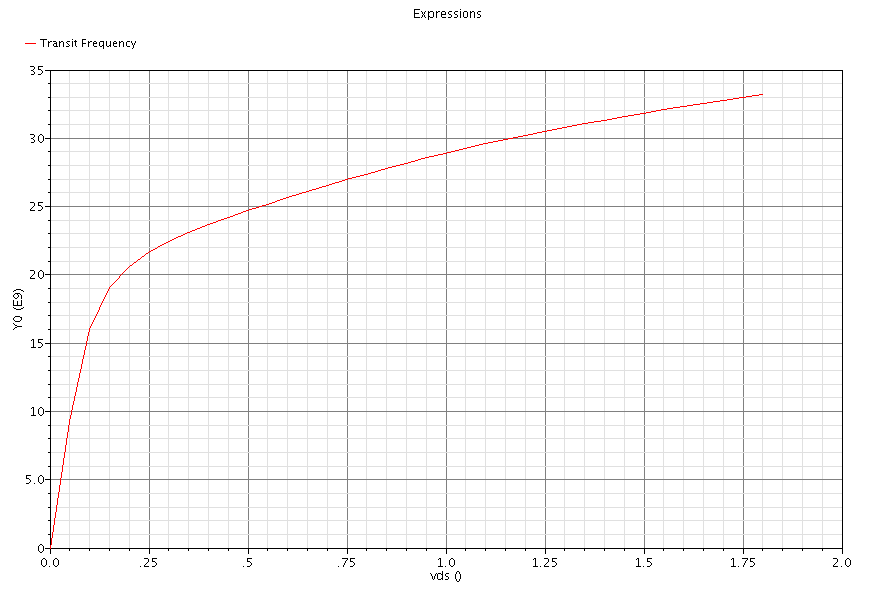
\includegraphics[width=\textwidth]{nmostransitfreq}
\caption{\transit\spc Dependence on $V_{ds}$} 
\label{fig:vdsdeptransit}
\end{figure}
From these graphs, it was decided that the minimum $V_{ds}$ required to obtain results close to the estimated results, while mainataining a reasonable output swing, was \SI{200}{\milli\volt}. In order to achieve this larger transistor drain to source voltage, the method used in Section \ref{sec:cascodebias} was used, to decrease the aspect ratio of the triode transistor. Once all of the transistor $V_{ds}$ voltages were raised to this value, the design parameters began to more closely resemble the calculated models.

Although increasing the $V_{ds}$ on the transistors did increase the gain significantly, this change was not enough for the design to meet the loop gain requirements. In order to increase the gain, the \gmid\spc of the transistors was increased to 20. After making this change, the loop gain specification was met, but the loop crossover frequency was only about \SI{16}{\mega\hertz}, well below the specified requirements. From Equation \ref{eq:cltotexact}, the crossover frequency is only dependent on the parasitics at the load node. In examining the capacitances at the load, it was noticed that the load capacitance contribution from the PMOS was much larger than that from the NMOS. Based on this observation, the width of the load PMOS was reduced in an effort to decrease the load capacitance. A reduction in transistor width while maintaining the same bias current results in a decrease in the transistor \gmid\spc. In the case of the PMOS load, a reduction in \gmid\spc to \SI{15}{\per\volt} was observed. While this modification did increase the crossover frequency of the OTA, it was still not high enough to meet specifications. Further reductions in the load \gmid\spc had little effect on the crossover frequency and caused sharp drops in gain, so the \gmid\spc was not modified any further. In order to meet the required crossover frequency, the $g_{m}$ of all transistors was increased to \SI{4.8}{\milli\siemens}. After this modification, the loop crossover frequency met specification. In retrospect, a much better knob to use would have been the \gmid\spc of the input NMOS transistor. Although the parasitics from the load transistors do reduce the crossover frequency, they are still a small percentage of the second stage sampling capacitance, which dominates the load capacitance. The size of the feedback capacitor is on the same order as the input parasitics, so changes in the input parasitics can have a much larger effect on the feedback factor of the OTA. Unfortunately, this realization was not made until after the design had already been checked out. This optimization will be assessed in future modifications to the OTA.

After overcoming these two major design challenges, the OTA was meeting the loop gain and loop crossover frequency specifications. Further simulations showed that the noise specification was also being met, so the rest of the simulations described in Section \ref{sec:otatests} were performed in order to fully characterize the OTA. The following section will present the results from all of these simulations.
\section{OTA Simulation Results}
This section summarizes the simulation results from the OTA tests described in \ref{sec:otatests}. These results include those from the \textit{stb} analysis, the DC output swing analysis, the AC noise simulation, and the transient simulation used to verify the CMFB network operation. This section will conclude with an overview of device parameters and performance results.
\subsection{STB Results}
The \textit{stb} analysis allowed for loop gain and phase measurements while taking into account the effect of the feedback network on the OTA. Figure \ref{fig:otastbresult} shows the results from this analysis. 
\begin{figure}[htbp]
\centering
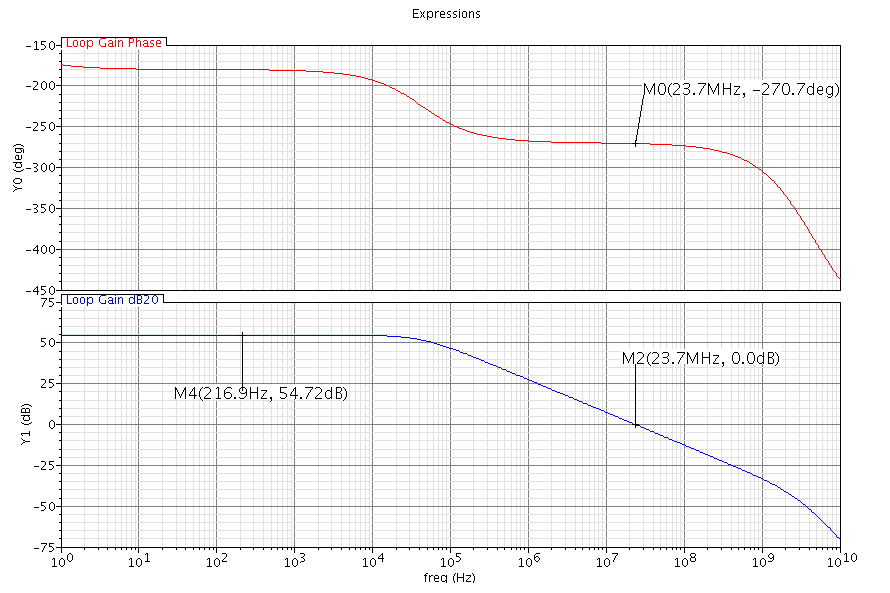
\includegraphics[width=\textwidth]{OTAloopgain}
\caption{STB Analysis Results} 
\label{fig:otastbresult}
\end{figure}
From this graph, the final loop gain is \SI{54.7}{\decibel} and the loop crossover frequency is \SI{23.7}{\mega\hertz}. In addition, the phase margin is \SI{89.3}{\degree}. All of these values are above their specified values.
\subsection{Output Swing}
Figure \ref{fig:otaoutputswing} shows the results from the output swing simulations. 
\begin{figure}[htbp]
\centering
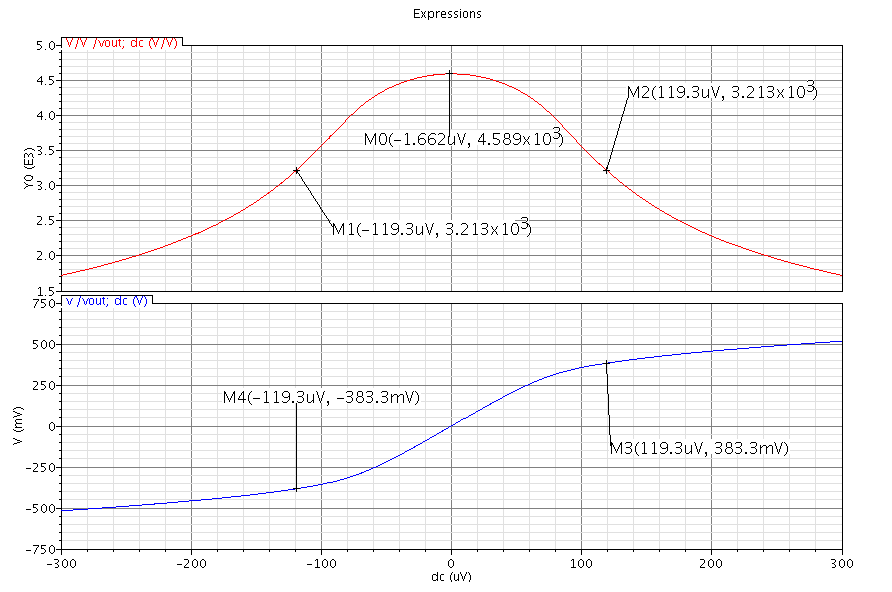
\includegraphics[width=\textwidth]{OTAoutputswing}
\caption{DC Output Swing Results} 
\label{fig:otaoutputswing}
\end{figure}
The peak open-loop gain is 4590. A reduction of 30\% of this value is a gain of 3213. The output voltage values at which the gain reaches 3213 are \SI{-383.3}{\milli\volt} and \SI{383.3}{\milli\volt}. This results in a total output swing of \SI{766.6}{\milli\volt}. This value is below the targeted output swing of \SI{1}{\volt}. An output swing of this value allows for approximately \nicefrac{1}{4} LSB of comparator offset. It was decided that with careful comparator design this tighter constraint could be met, so the output swing was deemed acceptable.
\subsection{OTA Noise}
Figure \ref{fig:otanoise} shows the results from the OTA AC noise simulations.
\begin{figure}[htbp]
\centering
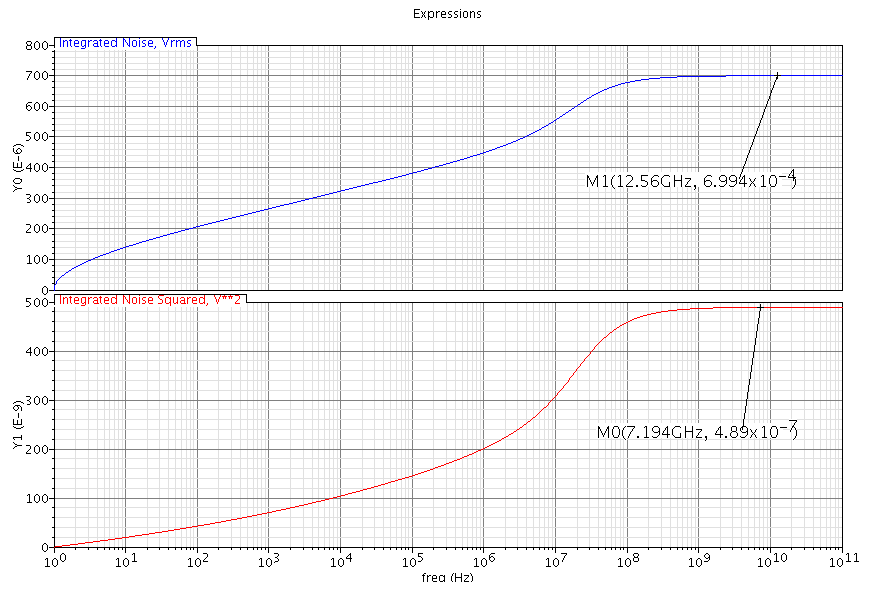
\includegraphics[width=\textwidth]{OTAnoise}
\caption{AC Noise Results} 
\label{fig:otanoise}
\end{figure}
The measured OTA output noise of \SI{699}{\micro\volt_{rms}} is still well below the maximum \SI{1.5}{\milli\volt_{rms}} allowed for in Table \ref{tab:maxoutputnoise}. This value is, however, well above the expected value calculated from \ref{eq:cascoutputnoise}. This is likely because the additional common-gate transistor causes much larger noise voltage on the output than allowed for by this equation. A better estimate would include the effects of the additional cascode stage and the additional gain it contributes to the common-source noise contribution. This calculation was not updated since the output noise was well within its limits.
\subsection{Real CMFB Transient Simulation}
In order to validate the operation of the passive CMFB network, a transiet simulation was performed. This transient simulation applied a sinusoidal input to the OTA and the output common-mode voltage was observed. Figure \ref{fig:cmfbresult} shows the output common-mode voltage measurements.
\begin{figure}[htbp]
\centering
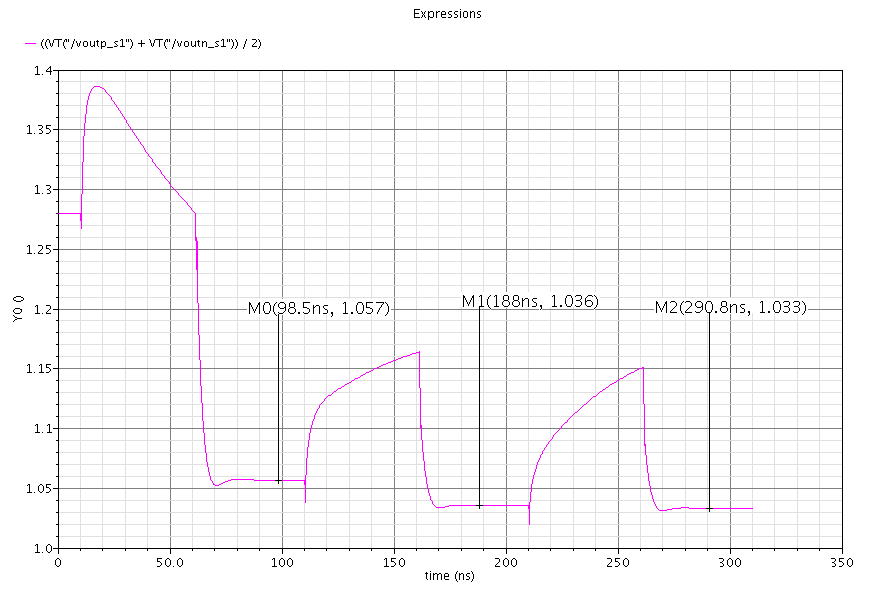
\includegraphics[width=\textwidth]{OTAcmfb}
\caption{Output Common-Mode Voltage Transient Simulation Results} 
\label{fig:cmfbresult}
\end{figure}
The deviations from the desired common-mode voltage observed occur during the $\phi_{1}$ clock phase and are the reason the OTA can only be active in the $\phi_{2}$ phase. While the OTA is in its active phase, the output common-mode agrees well with the desired common-mode voltage of \SI{1}{\volt}.
\subsection{Summary of OTA Simulation Results}
The measurements presented here show that the OTA achieved the performance desired for the ADC to achieve its performance specifications. Table \ref{tab:finalotadesign} summarizes the important design parameters, as well as the simulation results. Note that an additional transistor parameters had to be added to represent the PMOS load with different \gmid. Note also that $I_{total}$ is the total current used by the OTA, including additional current for the biasing circuits.
\begin{table}[htbp]
\begin{center}
\begin{tabular}{|l|r|}
\hline
Parameter & Value \\ \hline
$g_{m}/I_{d}$ & \SI{20}{\per\volt} \\ \hline
$(g_{m}/I_{d})_{PMOS,load}$ & \SI{15}{\per\volt} \\ \hline
$g_{m}$ & \SI{4.8}{\milli\siemens} \\ \hline
$I_{d}$ & \SI{694}{\micro\ampere} \\ \hline
$W_{PMOS}$ & \SI{280.7}{\micro\meter} \\ \hline
$W_{PMOS,load}$ & \SI{81.5}{\micro\meter} \\ \hline
$W_{NMOS}$ & \SI{92.5}{\micro\meter} \\ \hline
Loop gain & \SI{54.7}{\decibel} \\ \hline
$f_{c}$ & \SI{23.7}{\mega\hertz} \\ \hline
Phase Margin & \SI{89.3}{\degree} \\ \hline
Power & \SI{1.25}{\milli\watt} \\ \hline
Noise & \SI{699}{\micro\volt_{rms}} \\ \hline
\end{tabular}
\caption{Final OTA Design Parameters and Results}
\label{tab:finalotadesign}
\end{center}
\end{table}
\section{ADC Simulation Results With Integrated OTA}
Once the OTA performance was deemed acceptable, the next step was to perform the simulations outlined in Section \ref{sec:adcsimulations} on the differential ADC design with the transistor-level OTA model in place of the ideal OTA model. This section provides a summary of these results.

The first check for the ADC was a transient settling test. Since the performance of the OTA directly impacts the settling performance of the output to the second stage, ensuring that this test met its requirements was a very important step in verifying the OTA integration. Figures \ref{fig:tranotapos} and \ref{fig:tranotaneg} show the results from the transient simulation.
\begin{figure}[htbp]
\centering
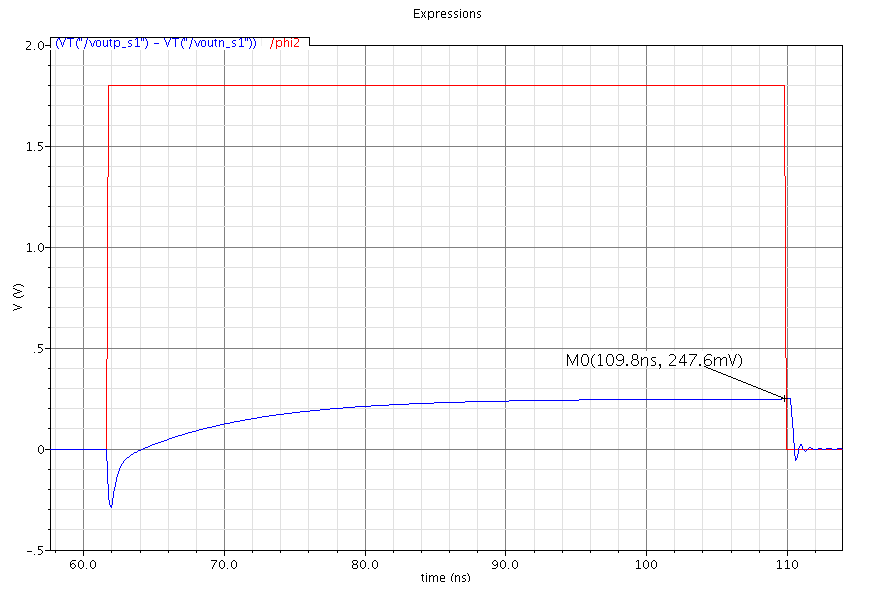
\includegraphics[width=\textwidth]{SAR_settlingfullpos}
\caption{Transient Settling of ADC With Real OTA Design With Full-Scale Positive Input Voltage} 
\label{fig:tranotapos}
\end{figure}
\begin{figure}[htbp]
\centering
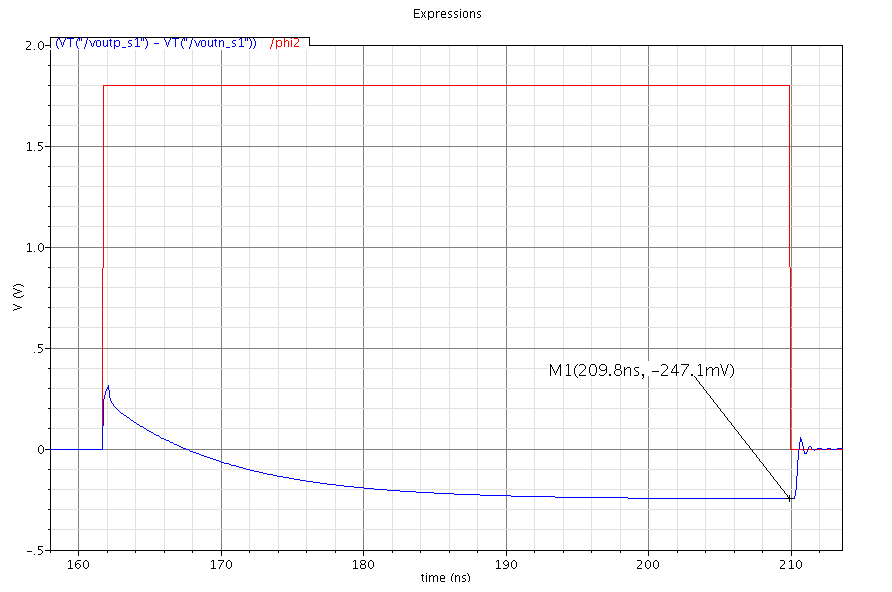
\includegraphics[width=\textwidth]{SAR_settlingfullneg}
\caption{Transient Settling of ADC With Real OTA Design With Full-Scale Negative Input Voltage} 
\label{fig:tranotaneg}
\end{figure}
In the case of the positive input, the settling error is \SI{-2.4}{\milli\volt}. In the case of the negative input, the transient settling error is \SI{2.9}{\milli\volt}. In both of these cases, the settling error is within the maximum settling error envelope.

Next, the full DFT simulation could be performed to measure the SQDR of the ADC. Figure \ref{fig:realotasqdr} shows the results from this simulation. 
\begin{figure}[htbp]
\centering
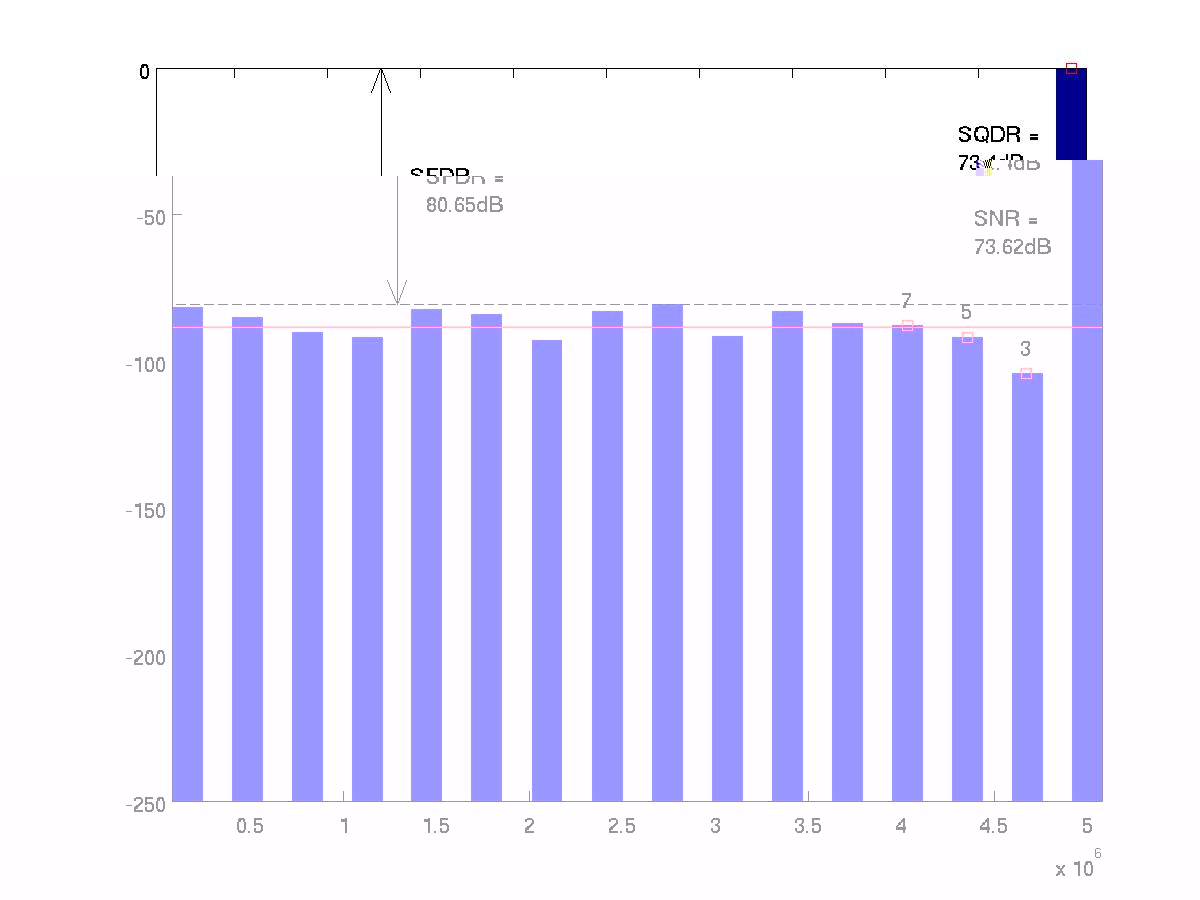
\includegraphics[width=\textwidth]{real_ota_diff_two_stage_douttotal_fft}
\caption{DFT of ADC With Real OTA Design } 
\label{fig:realotasqdr}
\end{figure}
The obtained SQDR was \SI{73.4}{\decibel}, a slight degradation from the ideal simulations. This degradation is expected, however, since simulations involving real transistors will have additional non-linearities that are not present in the ideal model. In addition, the SQDR is still very close to the ideal 12-bit SQDR, so this result was considered acceptable.

After performing the SQDR simulations, the noise performance of the entire ADC could be simulated. Only the AC noise in the hold phase and the PNOISE simulations needed to be rerun. Since the OTA is not active in the sampling phase, the OTA does not contribute to the output noise in that phase. Figure \ref{fig:otaholdnoise} is a graph of the simulated ADC noise in the hold phase.
\begin{figure}[htbp]
\centering
\includegraphics[width=\textwidth]{OTAholdnoise}
\caption{AC Noise During Hold Phase of ADC With Real OTA } 
\label{fig:otaholdnoise}
\end{figure}
The total output noise during the hold phase is \SI{723}{\micro\volt_{rms}}, which is in good agreement with the simulations performed only on the OTA model. The additional output noise is likely contributed from the switches. Once again, the output noise in the hold phase is well within budget. Table \ref{tab:acnoisesummaryrealota} summarizes the results from the AC noise simulation.
\begin{table}[htbp]
\begin{center}
\begin{tabularx}{\linewidth}{|l|X|X|X|X|}
\hline
Setup & AC Sampling Noise (\si{\milli\volt_{rms}}) & Total AC Hold Noise  (\si{\milli\volt_{rms}}) & AC Total Noise  (\si{\milli\volt_{rms}}) \\ \hline
Simulation & 1.52 & 0.72 & 1.68 \\ \hline
Calculation & 1.51 & 0.34 & 1.55 \\ \hline
Design Target & 1.51 & 1.52 & 2.15 \\ \hline
Error (\%) & 0.22 & 114.19 & 8.36 \\ \hline
Headroom (\%) & -0.22 & 52.52 & 21.75 \\ \hline
\end{tabularx}
\caption{AC Noise Summary With Real OTA}
\label{tab:acnoisesummaryrealota}
\end{center}
\end{table}

After obtaining AC noise simulations that were within budget, the PNOISE simulation was run to ensure good agreement between AC noise and PNOISE simulations. The graph from the PNOISE simulation is shown in Figure \ref{fig:pnoiserealota}
\begin{figure}[htbp]
\centering
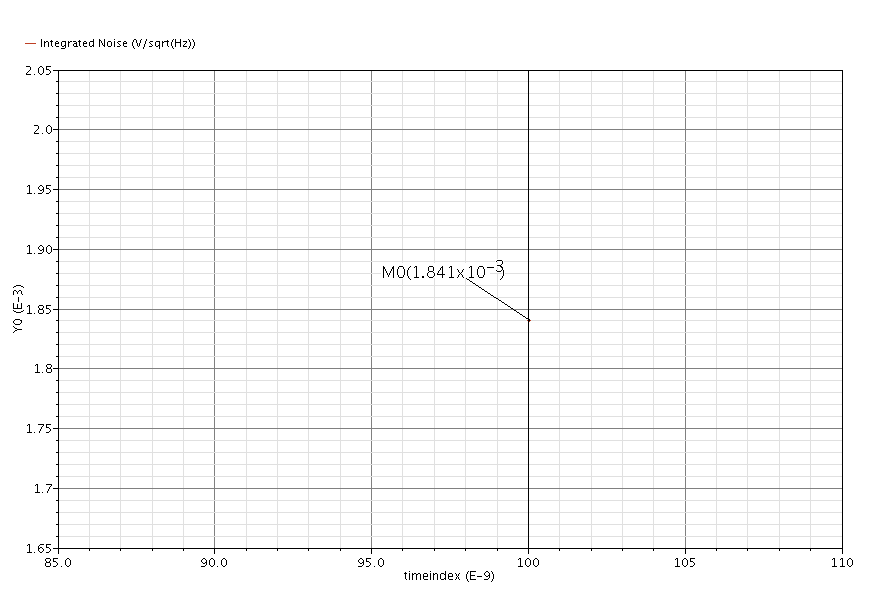
\includegraphics[width=\textwidth]{SAR_realota_pnoise}
\caption{PNOISE Simulation Results of ADC With Real OTA } 
\label{fig:pnoiserealota}
\end{figure}
While the PNOISE results are higher than that obtained from the AC noise simulations, the results are still within 20\% of each other. This level of agreement was considered acceptable for the noise simulations. Table \ref{tab:pnoisesummaryrealota} compares the results of the PNOISE simulation with the calculated values as well as the obtained AC noise measurements.
\begin{table}[htbp]
\begin{center}
\begin{tabularx}{\linewidth}{|l|X|X|X|}
\hline
Differential Noise &  &  &  \\ \hline
Setup & Total Noise Power (\si{\milli\volt_{rms}}) & Error vs Calculation (\%) & Error vs AC Simulation (\%) \\ \hline
PNOISE Simulations & \multicolumn{1}{r|}{1.84} & \multicolumn{1}{r|}{18.75} & \multicolumn{1}{r|}{9.58} \\ \hline
\end{tabularx}
\caption{ADC With Real OTA PNOISE Output Noise Summary}
\label{tab:pnoisesummaryrealota}
\end{center}
\end{table}

After obtaining acceptable results frm the noise simulation, the power consumption of the design could be simulated. Table \ref{tab:powerconsumptionrealota} summarizes the simulated average total current consumption and the contribution to the total from different circuit blocks.
\begin{table}[htbp]
\begin{center}
\begin{tabular}{|l|l|l|}
\hline
Circuit Block & Current (\si{\micro\ampere}) & Percent of Total \\ \hline
OTA & \SI{694}{\micro\ampere} & {80.98} \\ \hline
Digital logic and SAR capacitors & \SI{163}{\micro\ampere} & {19.02} \\ \hline
Total & \SI{857}{\micro\ampere} &  \\ \hline
\end{tabular}
\end{center}
\caption{ADC Power Consumption Summary}
\label{tab:powerconsumptionrealota}
\end{table}
From this average current, the average power consumption was calculated to be \SI{1.54}{\milli\watt}. 

As in the case of previous simulations, the results from the SQDR and noise simulations could be combined to obtain an SNDR and ENOB. Additionally, the ENOB, sampling frequency, and power consumption numbers could be combined to obtain the final FOM of the design. Since the PNOISE simulation produced the highest output noise, its value was used for the SNDR calculation. The SNDR calculated using these parameters was:
\begin{equation}
\label{eq:sndrdiffrealota}
SNDR = \SI{71.4}{\decibel}
\end{equation}
From Equation \ref{eq:sndridealdiff}, the ENOB is calculated to be 11.56 bits, which is still very close to an ideal 12-bit ADC performance.  Using Equation \ref{eq:fom}, the FOM for this design was calculated to be:
\begin{align}
\label{eq:fomrealota}
FOM &= \dfrac{\SI{1.54}{\milli\watt}}{\SI{10}{\mega\hertz}\cdot 2^{11.56}} \\[0.5em]
	&= 51\dfrac{\si{\femto\joule}}{\textnormal{conv-step}}
\end{align}
This number compares favorably with that obtained in other SAR-based pipeline designs~\cite{murmannadcsurvey}.

